\section{Implementation}
\label{sec:eval}

The implementation of the three algorithms to obtain performance results
was done using the C++ programming language along with the Message
Passing Interface standard (MPI).  The experiments were run on a 16 node
cluster of $64$-bit Xeon machines using $4$ cores on each node.
Each machine in the cluster runs the Linux operating system CentOS $6.x$.
The machines are connected to each other through a $10$Gbps local area
network. The complete implementation is approximately $2$K lines of code
and can be found at
https://github.com/shreya-68/Consensus/tree/master/MPI. A basic
synchronous peer-to-peer network framework was set up on top of which
the algorithms were implemented.

\subsection{Input}
The input into the system is size of the network, i.e., total number of processes, along with the input value for each of the processes for achieving consensus. The ratio of number of byzantine processes to the number of good processes is provided as well along with a specified byzantine behavior (see Section \ref{sec:behavior}). This behavior allows the byzantine processes to decide which values to send at every round of the protocol. 

\subsection{Output}
The output is the number of rounds carried out, latency in terms of CPU time utilization and elapsed real time, number of messages/bits sent per process, and the final decision value of each process. 

\subsection{Testing parameters}
For testing the three algorithms, the number of processes $(n)$ lies in the range $4$ to $64$ on a cluster of $1$ to $16$ machines. The number of faults $(f)$ lies in the range $[0, n/3)$ for algorithms \textit{Pull-Push} and \textit{EIG}, and in the range $[0, n/4)$ for algorithm \textit{Quorum}. The algorithms have been shown to be correct only in these respective ranges.

\subsection{Authentication of processes}
It was assumed that the channels are authenticated and each receiving entity knows the identity of the sender. The communication primitives provided by the MPI library implicitly provide this functionality and hence, a byzantine process cannot spoof their identity or hide it.

\subsection{Connection}
Each process in the peer-to-peer network had full knowledge about the network connection of other processes, i.e., the IP address and port number of the hosts it was connected to. Using the MPI library this is done by giving a unique ID to each process from $[0, n)$. The MPI point-to-point operations were used for sending and receiving messages between (any) two processes. This behaves like a TCP connection and was used for reliable transfer of messages between hosts. It also guarantees order between messages but does not guarantee fairness.% The implementation does not make use of any shared resources.

\subsection{Synchronization}
To implement a synchronous model of communication, communicators have been used. They are essentially a group of processes. \texttt{MPI\_Barrier}, a synchronization operation provided by the MPI library, allows one to specify a group to wait on. A process blocks on this call until all processes in the specified group reach this call. To keep all the processes in the network synchronized after each phase, this routine is used whose group is set to the active processes in the network.

\subsection{Parallelization}
To allow programs to execute parts of the protocol that are independent of each other in parallel, MPI thread level support has been used. To further improve performance, non-blocking calls have been used in some places where, for example, the execution of next few instructions does not depend on the completion of a send call. The MPI implementation creates a system buffer to typically hold data in transit. This is useful when a process wants to receive messages sent to it by multiple other processes at a later time. This improves performance by allowing send-receive operations to be asynchronous. The non-blocking calls were used such that execution within a round became asynchronous but not between rounds so as to ensure correctness. To ensure that messages are not lost by the overflow of a system buffer, each message was given a unique tag number which corresponded to a unique system buffer.


\subsection{Byzantine behaviors}
\label{sec:behavior}
A process can display the following byzantine behaviors:
\begin{itemize}
    \item Crash failure: Processes may fail by stopping. Any good process that fails to send messages or aborts its execution is considered byzantine. This is a worst-case assumption to ensure correctness even if for any unknown reason a good process fails.
    \item Processes send conflicting data to different processes in the same round. Any data that is not the same or is null is said to be conflicting.
    \item Processes send arbitrary content or more messages than necessary. Byzantine processes may try to do so to choke the communication and flood the network or overload the requests that need to be answered.
    \item Denial of service: Byzantine processes may deny responding to requests from good processes or may not forward messages as required. 
\end{itemize}

\subsection{Fault tolerance against crash failures}
We assume that once a process suffers a crash failure, it cannot recover from it. An advantage of using TCP connections was that it allowed failure discovery in the case of a crash failure. If a process failed before the start of a phase, no other process would be able to establish a connection with it which led to failure discovery. If a process crashed within a phase, the wait groups helped in detecting the failure by using a timeout mechanism. Each phase had to be completed within a certain amount of time and if all the processes did not reach the synchronization operation within that allotted time, it indicated a process failure and the other processes proceeded with the next phase. This mechanism worked since we were not dealing with more than $64$ processes and by running the system multiple times we could determine a timeout value that allowed alive processes to finish the phase with high probability. An alternative to this method was sending an acknowledgement back but we refrained from using this method since that meant dealing with twice the number of messages, which added unnecessary overhead for our testing purposes. 

\subsection{Message format}
Each message sent over the network was an array of bytes of the following form:
\begin{equation*}
    \mathtt{LENGTH}, \mathtt{PHASE}, \mathtt{MESSAGE}
\end{equation*}
The $\mathtt{LENGTH}$ parameter indicated how many bytes of the message to parse. The $\mathtt{PHASE}$ parameter indicated which phase the message was sent during and also what its purpose in that phase is. As in the algorithm \textit{Pull-Push}, the pull phase sends messages of type `ANSWER', `ROUTE', `FORWARD' and so on. The format of the $\mathtt{MESSAGE}$ varied for each of the algorithms.


\section{Results}
\label{sec:results}

\subsection{Bit Complexity}
For the \textit{EIG} algorithm, from Fig. \ref{fig:eig}, we can see that as the network size increases the bit complexity increases as a cubic function in accordance with the theoretical Big `O' complexity of $O(n^3 logn)$, where $n$ is the size of the network. This is a major improvement from classic deterministic algorithms that have very high polynomial growth. On a linear scale we note that the fault ratio affects the bit complexity by a factor of $n$. This is because with a higher ratio, faulty processes try to dominate the number of bits a good process receives by claiming all processes are byzantine in every round. They send $n^2$ bits of information in every round to every other process, whereas good processes send only $n*k$ bits of information. As the number of processes start to increase, the trends for each of the fault ratios becomes similar. However, for small networks, the bit complexity is quite diverse for different fault ratios. This shows that for systems with high variable size of the network, any fault ratio will affect the bandwidth consumption in a similar manner but, for small networks with varying fault ratios, the bandwidth consumption could be affected greatly.   
\begin{figure}[ht]
 \centering
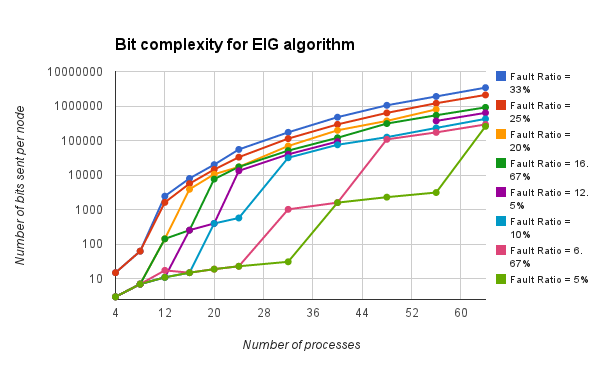
\includegraphics[scale=0.4]{eig}
\caption{Performance results for EIG algorithm (Log Scale)}
 \label{fig:eig}
\vspace{-2mm}
\end{figure}

%\begin{figure}[ht]
% \centering
%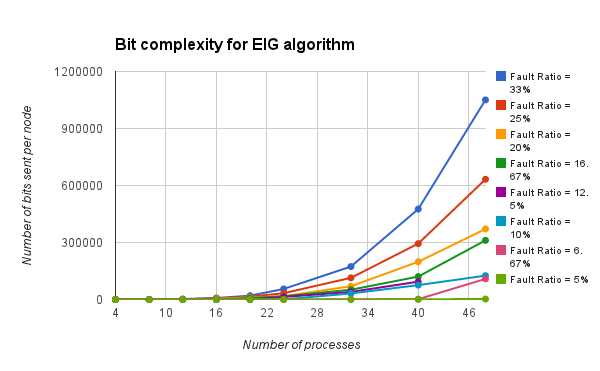
\includegraphics[scale=0.4]{eignolog}
%\caption{Consensus results for EIG algorithm}
% \label{fig:eignolog}
%\end{figure}
For the \textit{Pull-Push} algorithm, as the network size increases the bit complexity displays a poly-logarithmic growth. This can be seen in Fig. \ref{fig:pull_push}. The growth trend is similar for all fault ratios for small and larger networks. The increase in number of faults has an effect on the number of bits sent per process but only by a constant factor. This can be attributed to the fact that in the protocol, even if byzantine processes try to send conflicting values and a large number of them to samplers for the purpose of flooding, the samplers do not receive enough of them to forward these messages further in the protocol. Also note that for networks with $logn$ remaining the same, the bits sent per process is the same and it only changes at network sizes that are powers of $2$. This is because good processes only communicate with samplers of size $logn$. Hence, for larger networks, increasing the size of the network by less than $100\%$ will not affect the bandwidth consumption.
\begin{figure}[ht]
 \centering
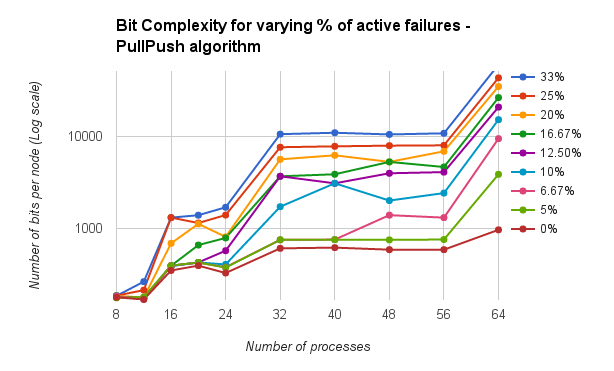
\includegraphics[scale=0.4]{pull_push}
\caption{Performance results for Pull-Push algorithm (Log scale)}
 \label{fig:pull_push}
\vspace{-2mm}
\end{figure}

From Figure \ref{fig:quorum}, algorithm \textit{Quorum} shows very high bits per process communication even for small networks. It increases rapidly as the network size increases. The reason for this is that \textit{Graded broadcast} requires all-to-all communication between processes and the protocol requires processes to run a deterministic byzantine agreement protocol for every subset of a committee in Stage $2$ of the protocol. The fault ratios do not have much of an effect on the communication costs. Byzantine processes are unable to increase bits on the network by participating in more sub-protocols than the algorithm requires since membership in a sub-protocol is dictated by their ID, which is fixed. Hence, more number of processes are unable to influence the communication cost greatly which is already high.  
\begin{figure}[ht]
 \centering
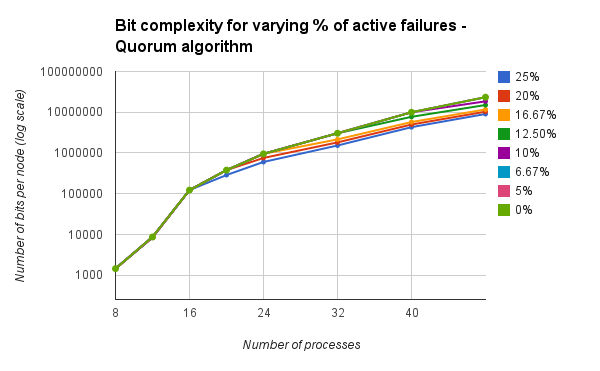
\includegraphics[scale=0.4]{quorum}
\caption{Performance results for Quorum algorithm (Log scale)}
 \label{fig:quorum}
\vspace{-2mm}
\end{figure}

Each of our algorithms for every configuration was run multiple times. In the analysis, each data point is an average over $5$ independent runs and we obtained confidence intervals for each of them. The confidence interval for algorithm \textit{Pull-Push} was $\pm 1\%$, for algorithm \textit{EIG} - $\pm 0.1\%$, and $\pm 0.5\%$ for algorithm \textit{Quorum}.

\subsection{Comparison}
For large networks ($n > 64$), we vary the ratio of faults to the number of processes ($f/n$), which lies in the range $[0, 1/3)$ for algorithms \textit{EIG} and \textit{Pull-Push}, and in the range $[0, 1/4)$ for algorithm \textit{Quorum}.
        As can be seen from Fig. \ref{fig:comp}, the algorithm \textit{Pull-Push} performs much better than the other algorithms for any fault percentage.

        Next, we modify the \textit{EIG} protocol a little to require that instead of sending the complete byzantine list every time, from round $4$ onwards only the changes to this list be sent in every round. We are motivated to do so since sending information about the existence of a process in the suspected byzantine list of another process in every round seems redundant. This does not change the correctness of the algorithm since all the good processes send the same changes to every other process in a round and in the next round the confirmation mechanism would confirm these updated lists. The rest of the algorithm works in the same way. Even though this does not change the communication complexity in the worst case, it overall reduces the communication bits as good processes would send a bit for every suspected byzantine process only in any one of the rounds instead of every round. This modified version of the algorithm performs much better. For small ratios, since the number of rounds is small, the number of bits sent per process remains the same. But, as the ratio increases, it varies greatly from the performance of algorithm \textit{EIG}.
\begin{figure}[ht]
 \centering
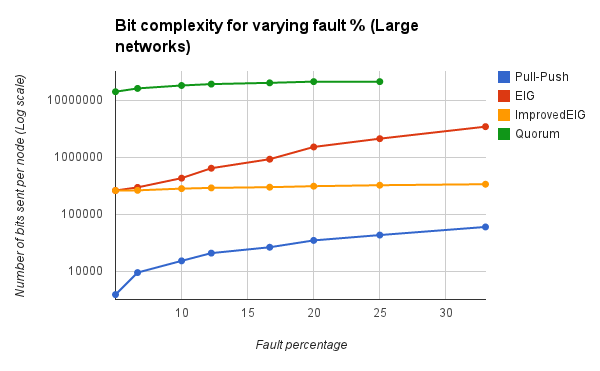
\includegraphics[scale=0.4]{LargeNetBit}
\caption{Comparison for large networks}
 \label{fig:comp}
\vspace{-2mm}
\end{figure}

\begin{figure}[ht]
 \centering
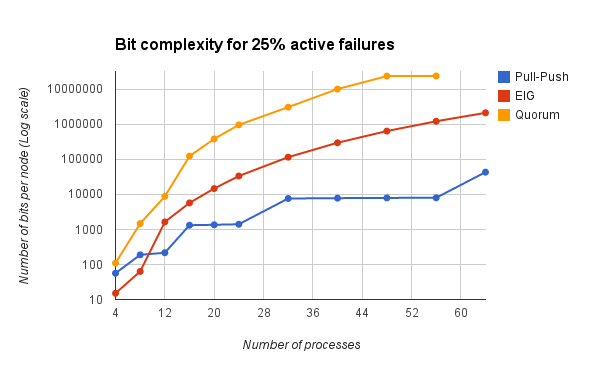
\includegraphics[scale=0.4]{Fault25}
\caption{Comparison for high \% of faults}
 \label{fig:fault25}
\vspace{-2mm}
\end{figure}

\begin{figure}[ht]
 \centering
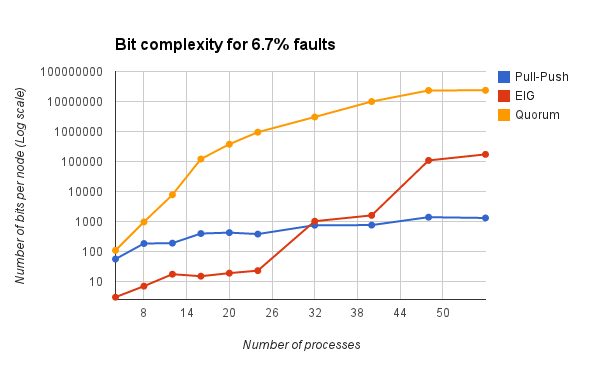
\includegraphics[scale=0.4]{Fault667}
\caption{Comparison for low \% of faults}
 \label{fig:fault667}
\vspace{-2mm}
\end{figure}

\begin{figure}[ht]
 \centering
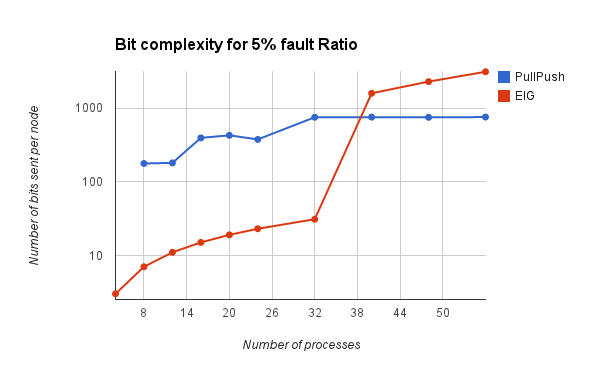
\includegraphics[scale=0.4]{Fault5}
\caption{Comparison for low \% of faults}
 \label{fig:fault5}
\vspace{-2mm}
\end{figure}

For small networks ($n < 40$), if the fault ratio is small and in the range $[0, 1/15)$, Figs. \ref{fig:fault667} and \ref{fig:fault5} show that algorithm \textit{EIG} performs much better than any of the other algorithms. This is simply because only the first three rounds of this algorithm will be executed and since the ratio is small, a simple broadcast is sufficient to gather all the information. \textit{Pull-Push} and \textit{Quorum}, which are more complex algorithms, perform worse in such scenarios. Fig. \ref{fig:fault25} shows that for higher fault ratios and any network size, algorithm \textit{Pull-Push} performs better.

    Depending on the system requirements such as how fast we want the information to reach the destination, bandwidth and so on, there were two mechanisms we used to send the messages. In an algorithm like \textit{Pull-Push}, where multiple message packets may be sent to the same process by a process in the same round, one could marshal all the packets into one packet and then send it. This obviously comes at the cost of parallelization where one has to first wait to receive all the messages from the previous round, perform operations and then send out messages all at once. While the number of messages sent per process changed when using the latter method, the number of bits sent remained the same.

%The difference in the number of messages sent for the two mechanisms can be seen in Fig. \ref{fig:opt}.
%\begin{figure}[h]
% \centering
%\includegraphics[scale=0.55]{optimized}
%\caption{ EIG algorithm when messages are grouped before sending}
% \label{fig:opt}
%\end{figure}

\subsection{Round Complexity}
Round complexity is the number of phases that have to be executed sequentially by a process and one cannot parallelize these phases. For example, in algorithm \textit{EIG}, a round consists of broadcast of messages at the same level $i$ in the \textit{EIG} tree of each process. For algorithm \textit{Quorum}, a round consists of broadcast of messages during a particular sub-protocol. There are two ways to analyze the round complexity of this algorithm. The first is that each of the sub-protocols $S_i^j$ could be executed in parallel since none of these sub-protocols are dependent on each other. Hence, all of them together make one round. But, if parallel execution of these sub-protocols is not possible due to resource constraints then each of them is an independent round. We implemented the algorithm to run the sub-protocols in parallel since that improved the round complexity. For algorithm \textit{Pull-Push}, the push phase makes one round and sending, routing and answering in the pull phase form independent rounds.

\begin{figure}[ht]
 \centering
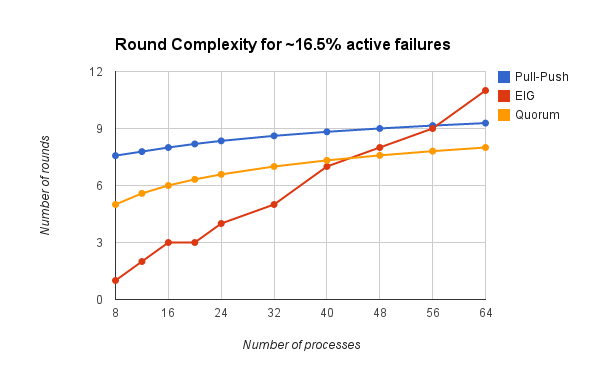
\includegraphics[scale=0.4]{Round16}
\caption{Round Complexity comparison}
 \label{fig:round16}
\vspace{-2mm}
\end{figure}

\begin{figure}[ht]
 \centering
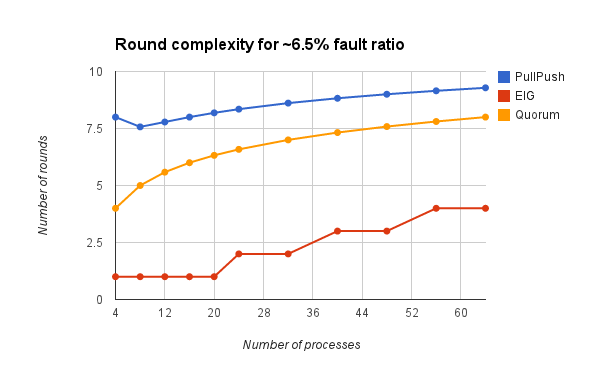
\includegraphics[scale=0.4]{Round6}
\caption{Round Complexity comparison}
 \label{fig:round6}
\vspace{-2mm}
\end{figure}

A comparison of the round complexities can be seen in Figs. \ref{fig:round16} and \ref{fig:round6} for fault percentage $~16.5\%$ and $~6.5\%$, respectively. We can see that for a very small ratio of $~6.5\%$ the round complexity of \textit{EIG} is better but for larger ratios and larger networks $(n > 40)$ \textit{Quorum} performs better than the other two. 


\subsection{Latency}

For performance comparison of latency, we compare the total CPU times and elapsed real time.  The total CPU time is the sum of CPU time consumed by all of the CPUs utilized by an execution of an algorithm. If a program has parallel tasks, the total CPU time takes into account the time taken by each of the tasks. Elapsed real time is simply the time taken from the start of a computer program until it terminates as measured by an ordinary clock. From Figures \ref{fig:cpu} and \ref{fig:elapsed}, we see that CPU time utilization and elapsed real time of \textit{EIG} increases rapidly and it is a lot slower compared to the other two algorithms. If we look at the elapsed real time, we can see that algorithm \textit{Quorum} remains the fastest throughout. This is because \textit{Quorum} is highly parallel. The trade-off here is that the CPU time utilization of \textit{Quorum} is a lot more than that of \textit{Pull-Push}. This trend is maintained for all fault ratios.

\begin{figure}[ht]
 \centering
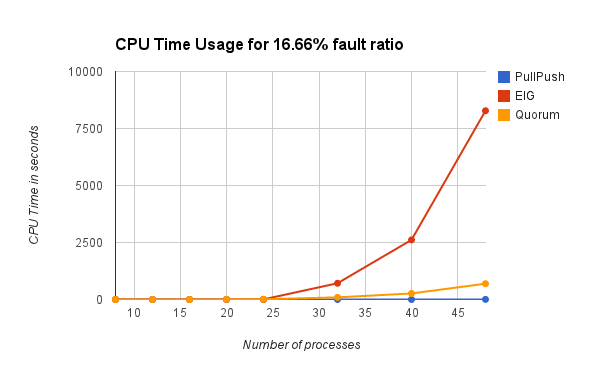
\includegraphics[scale=0.4]{cpu16}
\caption{CPU time utilization comparison}
 \label{fig:cpu}
\vspace{-2mm}
\end{figure}

\begin{figure}[ht]
 \centering
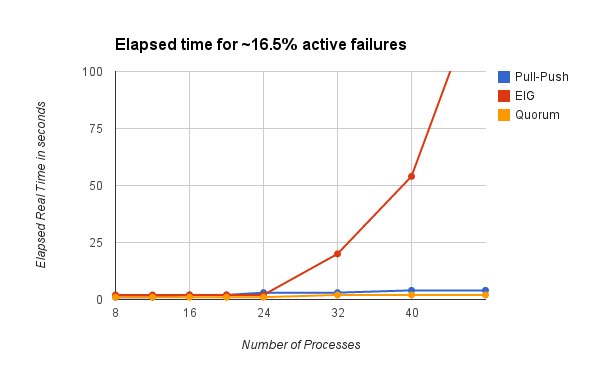
\includegraphics[scale=0.4]{elapsed16}
\caption{Elapsed real time comparison}
 \label{fig:elapsed}
\vspace{-2mm}
\end{figure}

%Fig. \ref{fig:time} the first mechanism for calculating time complexity of algorithm Quorum is used, where it is considered that all the subprotocols together form one round. This figure shows the algorithm Quorum gives better performance than algorithms EIG and Pull-Push as the number of processes in the network increases. Also, algorithm Pull-Push diverges in complexity due to increasing number of candidate strings that could be injected by the adversarial processes.

%Fig. \ref{fig:time_nopar}, shows a comparison of time complexities if each subprotocol in algorithm Quorum is treated as an individual round. In contrast to Fig. \ref{fig:time}, this figure clearly shows that the time complexity of algorithm Quorum increases rapidly, whereas for algorithms EIG and Pull-Push there is no drastic increase. Hence, if resources are limited and parallel processing of each subprotocol is not possible, algorithm Quorum does not give good performance.
%
%\begin{figure}[h]
% \centering
%\includegraphics[scale=0.55]{time_nopar}
%\caption{Time Complexity comparison no parallel execution}
% \label{fig:time_nopar}
%\end{figure}



